%% 
%% Template article for cas-sc documentclass for 
%% double column output.
%%

\documentclass[a4paper,fleqn]{cas-sc}

\usepackage[authoryear,longnamesfirst]{natbib}
\usepackage{tikz}
\usetikzlibrary{positioning, arrows.meta, shapes}
\usepackage{float}
\usepackage{placeins}

%%%Author definitions
\def\tsc#1{\csdef{#1}{\textsc{\lowercase{#1}}\xspace}}
\tsc{BPM}
\tsc{BPS}
\tsc{DES}
\tsc{RL}
\tsc{LSTM}
\tsc{GRU}
%%%

\begin{document}
\let\WriteBookmarks\relax
\def\floatpagepagefraction{0.7}
\def\textpagefraction{.001}

% Short title
\shorttitle{Runtime Declarative To-Be Short-Term Simulation}

% Short author
\shortauthors{A. Mosquera}

% Main title of the paper
\title[mode=title]{Runtime Declarative To-Be Short-Term Simulation Pipeline}                      

% Optional title notes
\tnotemark[1]
\tnotetext[1]{This work specifies a modular runtime pipeline integrating declarative what-if design, deep generative models, and short-term discrete-event simulation for business processes.}

% First (and only) author
\author[1]{Andr\'es Mosquera}[
   role=Researcher,
]
\cormark[1]
\ead{andres.mosquera@example.org}

\affiliation[1]{organization={Universidad de los Andes},
    city={Bogot\'a},
    country={Colombia}}

% Corresponding author text
\cortext[cor1]{Corresponding author}

% Non-numbered note
\nonumnote{This article provides a white-box specification of a runtime
pipeline that integrates a declarative deep generative module,
an ongoing state computation engine, and a short-term simulation and
evaluation layer, targeting prescriptive what-if / To-Be analysis.}

% Abstract
\begin{abstract}
Prescriptive process monitoring and business process simulation are 
typically studied as separate problems: \emph{offline} what-if / To-Be
analysis based on synthetic or historical logs, and \emph{runtime}
monitoring and prediction based on the current execution state.
This article specifies an integrated
pipeline---the \emph{ShortTerm Declarative To-Be Integration Pipeline}
(ST-TOBE)---that connects three existing capabilities:
declarative, deep-learning-based what-if generation of To-Be BPMN models,
runtime reconstruction of partial process state, and short-term
discrete-event simulation and evaluation.

ST-TOBE starts from an original event log and a set of
declarative control-flow rules, trains (or reuses) LSTM/GRU models
to hallucinate traces that enforce those rules, discovers BPMN
AS-IS and TO-BE models, merges To-Be structure with AS-IS resource
and timing parameters, reconstructs the current partial state of
the process with respect to the TO-BE model, and runs
short-term simulations (Prosimos and BIMP) from that state.  
The resulting simulated logs and statistics are compared with
reference windows in the original data using event-, ongoing-, and
completion-based filters, yielding interpretable KPIs and visual
reports.

We describe the architecture, data contracts, configuration
parameters, and extensibility points in a white-box manner.
The goal is to make the interplay between
deep generative models, declarative constraints, BPMN discovery,
runtime state reconstruction, and short-term simulation 
transparent and reproducible, and to support future empirical
studies on runtime what-if / To-Be analysis under realistic,
resource-aware simulation settings.
\end{abstract}

% Highlights
\begin{highlights}
\item Provides a white-box specification of an integrated pipeline that combines declarative what-if / To-Be generation, runtime state reconstruction, and short-term simulation.
\item Describes the internal data flow between deep generative LSTM/GRU models, BPMN discovery, Prosimos/BIMP simulation, and an ongoing-state engine driven by N-gram indices and reachability graphs.
\item Defines a structured evaluation layer that compares short-term simulated behaviour of TO-BE models against reference logs using event, ongoing, and completion filters.
\end{highlights}

% Keywords
\begin{keywords}
Prescriptive process monitoring \sep
What-if / To-Be analysis \sep
Short-term simulation \sep
Declarative constraints \sep
BPMN \sep
Deep generative models \sep
Runtime process state
\end{keywords}

\maketitle

%========================================
\section{Introduction}
%========================================

Prescriptive process monitoring and business process simulation
have evolved along largely independent lines.  
Prescriptive approaches focus on triggering interventions or
recommending actions at runtime based on predictions and causal
reasoning \citep{Shoush2025IS,Shoush2024arXiv}, whereas simulation-based approaches support what-if and
To-Be analysis by exploring hypothetical changes to process models,
resource allocations, or demand patterns in an offline fashion.

Recent work in business process simulation and prescriptive
monitoring suggests a need to bridge these two views
\citep{Meneghello2025IS,Avramenko2025arXiv}.
On the one hand, simulation results should be grounded in realistic, 
data-driven models that reflect current execution conditions.
On the other hand, prescriptive decisions should be evaluated not only
in terms of predicted outcomes but also in terms of their impact on the
stochastic behaviour of the process over time.
This calls for infrastructures where
data-driven To-Be models, runtime state reconstruction, and
short-term simulation are combined in a single, coherent pipeline.

This article presents the \emph{ShortTerm Declarative To-Be Integration Pipeline}
(ST-TOBE), a runtime-oriented architecture that connects:
(i) a declarative deep generative pipeline that produces To-Be BPMN models,
(ii) an ongoing-state engine that reconstructs partial process state and
supports short-term simulation, and
(iii) an integration layer that orchestrates these components and evaluates
short-term behaviour against reference data.

Rather than introducing new prediction or simulation algorithms, the
contribution of this work is a \emph{white-box specification} of the
overall architecture: the data structures and file formats that link
the modules, the configuration parameters that govern their behaviour,
and the extension points that enable alternative implementations
\citep{Shoush2025IS}.
The resulting specification clarifies how legacy components (e.g., BIMP,
Prosimos, standard BPMN discovery) interact with newer ones
(e.g., deep generative models, declarative rules, ongoing-state
reconstruction, and short-term evaluation) in a runtime To-Be analysis setting.

The remainder of this article is structured as follows.
Section~\ref{sec:background} summarises the required background.
Section~\ref{sec:overview} provides a high-level overview of the
ST-TOBE architecture and data flow.
Section~\ref{sec:integration} details the
\emph{shorterm/con-to-be} integration and evaluation layer.
Section~\ref{sec:whitebox} consolidates the white-box
specification in terms of configuration, data contracts, and
extensibility.
Section~\ref{sec:discussion} discusses limitations and potential
extensions, and Section~\ref{sec:conclusion} concludes the paper.
Detailed specifications of the \emph{DeclarativeProcessSimulation}
and \emph{ongoing-bps-state-short-term} modules are provided in
Appendix~\ref{app:declarative_module} and Appendix~\ref{app:ongoing_module},
respectively.

%========================================
\section{Background}
\label{sec:background}
%========================================

This section briefly reviews the concepts that underpin the
ST-TOBE pipeline: 
(a) declarative what-if / To-Be analysis driven by deep
generative models, 
(b) runtime state reconstruction and short-term simulation, and 
(c) log-based short-term evaluation.

\subsection{Declarative what-if / To-Be analysis}

Declarative process analysis focuses on specifying and
enforcing business rules in terms of constraints on event
sequences, rather than prescribing a single, rigid control-flow
structure.
Constraints can capture ordering and frequency requirements or
forbid certain activities altogether.
In a what-if / To-Be setting, such constraints are used to
shape hypothetical future behaviour while preserving key
statistical properties of the observed log.

In the context of ST-TOBE, declarative rules are encoded in
\verb|rules.ini| files and use a compact syntax to express
patterns such as direct succession, eventual succession, forbidden
activities, required activities, and frequency variations.
Deep generative models (e.g., LSTM/GRU architectures) are trained
on the original event log and then guided by these rules to
generate synthetic traces that represent To-Be scenarios.

\subsection{Runtime state reconstruction and short-term simulation}

Runtime state reconstruction aims to infer, at a given cut-off
time, the \emph{partial state} of all ongoing process instances
\citep{ChapelaCampa2025TSC}.
Given an event log truncated at the cut-off, and a process model
with simulation parameters, the goal is to determine which
activities are currently running, which elements are enabled,
and how tokens are distributed over the control-flow graph.

Short-term simulation then uses this partial state as an initial
condition and projects the process forward over a limited
horizon \citep{Avramenko2025arXiv}.
Instead of simulating from an empty initial state, the engine
starts from the reconstructed marking and the set of ongoing
activities, thus capturing the influence of the current workload
and process history on near-future behaviour.

\subsection{Short-term evaluation with log-based filters}

To assess how well a short-term simulation reproduces the
behaviour of a real process, one can compare simulated and
reference logs over a given time window around the cut-off.
This comparison can focus on different aspects, such as:
(i) all events occurring in the window,
(ii) cases that remain ongoing at the cut-off time, or
(iii) cases that complete within the horizon.
By computing metrics such as precision, recall, and F1-score
for these subsets, one obtains interpretable indicators of
short-term realism that complement long-horizon To-Be analysis.

%========================================
\section{System overview}
\label{sec:overview}
%========================================

Figure~\ref{fig:architecture} illustrates the
ST-TOBE architecture.
Starting from an original event log and declarative rules, the
pipeline proceeds through an \emph{offline} To-Be
generation phase, followed by an \emph{online} ongoing-state
phase and a \emph{short-term evaluation} phase.

\FloatBarrier
\clearpage
\begin{figure}[H]
  \centering
  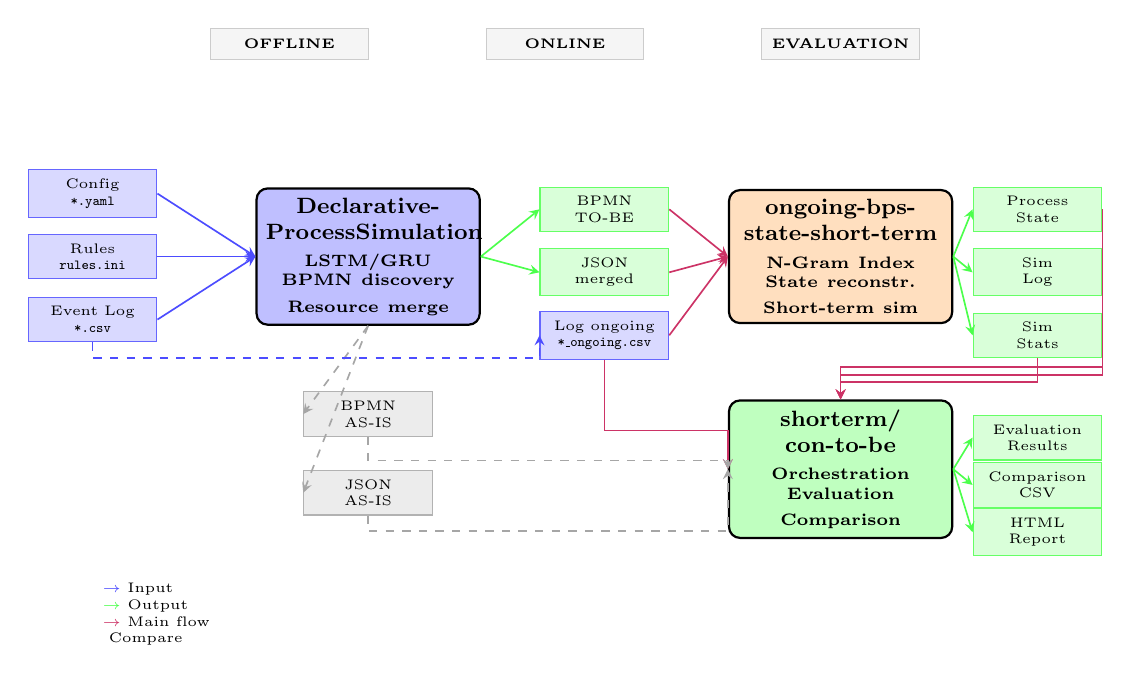
\begin{tikzpicture}[
    node distance=1cm and 1.5cm,
    module/.style={rectangle, rounded corners, draw=black, thick, 
                   minimum width=2.8cm, minimum height=1.6cm, 
                   text width=2.6cm, align=center, font=\footnotesize\bfseries},
    input/.style={rectangle, draw=blue!60, fill=blue!15, 
                  minimum width=1.6cm, minimum height=0.5cm, 
                  text width=1.4cm, align=center, font=\tiny},
    output/.style={rectangle, draw=green!60, fill=green!15, 
                   minimum width=1.6cm, minimum height=0.5cm, 
                   text width=1.4cm, align=center, font=\tiny},
    arrow/.style={->, >=stealth, semithick},
    phase/.style={rectangle, draw=gray!40, fill=gray!8, 
                  minimum width=2cm, minimum height=0.4cm, 
                  font=\tiny\bfseries, align=center}
  ]
    
    % Phase labels at top
    \node[phase] (phase1) at (-3.5, 3.2) {OFFLINE};
    \node[phase] (phase2) at (0, 3.2) {ONLINE};
    \node[phase] (phase3) at (3.5, 3.2) {EVALUATION};
    
    % Inputs to DeclarativeProcessSimulation (left side)
    \node[input] (config) at (-6, 1.3) {Config\\\texttt{*.yaml}};
    \node[input] (rules) at (-6, 0.5) {Rules\\\texttt{rules.ini}};
    \node[input] (log) at (-6, -0.3) {Event Log\\\texttt{*.csv}};
    
    % DeclarativeProcessSimulation module
    \node[module, fill=blue!25] (declarative) at (-2.5, 0.5) {
      Declarative-\\
      ProcessSimulation\\
      \vspace{0.1cm}
      \fontsize{6}{7}\selectfont
      LSTM/GRU\\
      BPMN discovery\\
      Resource merge
    };
    
    % Key outputs from DeclarativeProcessSimulation
    \node[output] (bpmn-tobe) at (0.5, 1.1) {BPMN\\TO-BE};
    \node[output] (json-merged) at (0.5, 0.3) {JSON\\merged};
    
    % Ongoing-bps-state-short-term module
    \node[module, fill=orange!25] (ongoing) at (3.5, 0.5) {
      ongoing-bps-\\
      state-short-term\\
      \vspace{0.1cm}
      \fontsize{6}{7}\selectfont
      N-Gram Index\\
      State reconstr.\\
      Short-term sim
    };
    
    % Log ongoing (external input)
    \node[input] (log-ongoing) at (0.5, -0.5) {Log ongoing\\\texttt{*\_ongoing.csv}};
    
    % Outputs from ongoing-bps-state
    \node[output] (state) at (6, 1.1) {Process\\State};
    \node[output] (sim-log) at (6, 0.3) {Sim\\Log};
    \node[output] (sim-stats) at (6, -0.5) {Sim\\Stats};
    
    % shorterm/con-to-be integration module
    \node[module, fill=green!25] (integration) at (3.5, -2.2) {
      shorterm/\\
      con-to-be\\
      \vspace{0.1cm}
      \fontsize{6}{7}\selectfont
      Orchestration\\
      Evaluation\\
      Comparison
    };
    
    % Final outputs
    \node[output] (eval-results) at (6, -1.8) {Evaluation\\Results};
    \node[output] (comparison) at (6, -2.4) {Comparison\\CSV};
    \node[output] (report) at (6, -3) {HTML\\Report};
    
    % AS-IS outputs for comparison
    \node[output, draw=gray!60, fill=gray!15] (bpmn-asis) at (-2.5, -1.5) {BPMN\\AS-IS};
    \node[output, draw=gray!60, fill=gray!15] (json-asis) at (-2.5, -2.5) {JSON\\AS-IS};
    
    % Arrows from inputs to DeclarativeProcessSimulation
    \draw[arrow, blue!70] (rules.east) -- (declarative.west);
    \draw[arrow, blue!70] (config.east) -- (declarative.west);
    \draw[arrow, blue!70] (log.east) -- (declarative.west);
    
    % Arrows from DeclarativeProcessSimulation to key outputs
    \draw[arrow, green!70] (declarative.east) -- (bpmn-tobe.west);
    \draw[arrow, green!70] (declarative.east) -- (json-merged.west);
    
    % Arrows from DeclarativeProcessSimulation to AS-IS outputs
    \draw[arrow, gray!70, dashed] (declarative.south) -- (bpmn-asis.west);
    \draw[arrow, gray!70, dashed] (declarative.south) -- (json-asis.west);
    
    % Arrow from log original to log ongoing
    \draw[arrow, blue!70, dashed] (log.south) -- ++(0,-0.2) -| (log-ongoing.west);
    
    % Arrows from outputs to ongoing-bps-state
    \draw[arrow, purple!80] (bpmn-tobe.east) -- (ongoing.west);
    \draw[arrow, purple!80] (json-merged.east) -- (ongoing.west);
    \draw[arrow, purple!80] (log-ongoing.east) -- (ongoing.west);
    
    % Arrows from ongoing-bps-state to outputs
    \draw[arrow, green!70] (ongoing.east) -- (state.west);
    \draw[arrow, green!70] (ongoing.east) -- (sim-log.west);
    \draw[arrow, green!70] (ongoing.east) -- (sim-stats.west);
    
    % Arrows from ongoing-bps-state outputs to integration
    \draw[arrow, purple!80] (state.east) -- ++(0,-2) -| (integration.north);
    \draw[arrow, purple!80] (sim-log.east) -- ++(0,-1.3) -| (integration.north);
    \draw[arrow, purple!80] (sim-stats.south) -- ++(0,-0.3) -| (integration.north);
    
    % Arrow from log-ongoing to integration
    \draw[arrow, purple!80] (log-ongoing.south) -- ++(0,-0.9) -| (integration.west);
    
    % Arrows from AS-IS outputs to integration
    \draw[arrow, gray!70, dashed] (bpmn-asis.south) -- ++(0,-0.3) -| (integration.west);
    \draw[arrow, gray!70, dashed] (json-asis.south) -- ++(0,-0.2) -| (integration.west);
    
    % Arrows from integration to final outputs
    \draw[arrow, green!70] (integration.east) -- (eval-results.west);
    \draw[arrow, green!70] (integration.east) -- (comparison.west);
    \draw[arrow, green!70] (integration.east) -- (report.west);
    
    % Legend (bottom left)
    \node[anchor=north west, font=\tiny] at (-6, -3.5) {
      \begin{tabular}{@{}l@{}}
        \textcolor{blue!70}{$\rightarrow$} Input\\
        \textcolor{green!70}{$\rightarrow$} Output\\
        \textcolor{purple!80}{$\rightarrow$} Main flow\\
        \textcolor{gray!70}{$\dashrightarrow$} Compare
      \end{tabular}
    };
    
  \end{tikzpicture}
  \caption{Conceptual architecture of the ShortTerm Declarative To-Be Integration Pipeline (ST-TOBE). 
           The pipeline integrates three main modules: DeclarativeProcessSimulation (offline phase), 
           ongoing-bps-state-short-term (online phase), and shorterm/con-to-be (evaluation and orchestration). 
           Solid arrows indicate main data flow; dashed arrows indicate comparison data.}
  \label{fig:architecture}
\end{figure}
\FloatBarrier

At this level, ST-TOBE can be seen as an orchestrated composition of:
a declarative, deep generative To-Be pipeline,
an ongoing-state engine for partial-state computation and short-term simulation,
and a layer that aggregates long-horizon and short-term evaluation artefacts
into integrated comparison and reporting outputs.

\subsection{Why ST-TOBE is runtime what-if / To-Be}

The taxonomy followed in the accompanying SLR distinguishes
\emph{As-Is} (descriptive), \emph{what-if} (scenario exploration), and
\emph{To-Be} (future design) models, together with \emph{runtime/online}
execution and \emph{short-term} simulation horizons
\citep{Meneghello2025IS,Middelhuis2025IS,Avramenko2025arXiv,ChapelaCampa2025TSC}.
ST-TOBE aligns with the \emph{runtime what-if / To-Be} quadrant because each
component in \verb|shorterm/con-to-be| is implemented to satisfy the
following characteristics.

\paragraph{To-Be design.}
Phase~1 of \verb|run_complete_integration.py| orchestrates the
\emph{DeclarativeProcessSimulation} pipeline to hallucinate traces with
LSTM/GRU models guided by declarative rule files (\verb|rules.ini|),
discover TO-BE BPMN structures, and merge AS-IS resources into the new
control-flow. These steps produce artefacts under
\verb|data/3.bps_tobe/| that explicitly encode the desired future model,
matching the definition of To-Be processes in runtime optimisation
studies such as \citep{Middelhuis2025IS}.

\paragraph{What-if exploration.}
The short-term evaluation scripts (\verb|evaluate_short_term_results.py|)
accept different combinations of reference windows, horizons, and rule
sets, allowing analysts to answer questions of the form ``what happens if
we enforce constraint set $X$ on log $Y$?''. Each invocation compares the
newly generated TO-BE artefacts against observed data, mirroring the
scenario-analysis role of runtime what-if simulators like
\citep{Meneghello2025IS}.

\paragraph{Runtime and online operation.}
Phases~2 and~3 consume the most recent \verb|*_ongoing.csv| files,
incrementally reconstructed partial states (\verb|process_state.json|),
and dynamically selected horizons. Because the orchestration reuses the
current process execution traces rather than historical, completed logs,
it operates online in the sense of \citep{ChapelaCampa2025TSC}: events are
processed as they arrive, and the integration can be re-run whenever the
state files are updated, keeping the analysis aligned with the live
process.

\paragraph{Simulation and short-term horizon.}
\verb|test_ongoing_only.py| and the delegated Prosimos runs execute
discrete-event simulations from the reconstructed marking, but only for a
limited horizon (default seven days) determined at runtime based on the
cut-off timestamp. This matches the definition of short-term simulation
from \citep{Avramenko2025arXiv}, where predictions start from the current
state instead of from an empty initial condition.

Taken together, these behaviours justify the terminology
``runtime what-if / To-Be short-term simulation pipeline'' used throughout
the paper: TO-BE artefacts are generated, explored, and validated against
live data through online, horizon-bounded simulations triggered directly
from the \verb|shorterm/con-to-be| orchestration scripts.

\subsection{Positioning with respect to existing components}

The \emph{ShortTerm Declarative To-Be Integration Pipeline} (ST-TOBE)
builds upon two pre-existing and independent systems:
(i) the \emph{DeclarativeProcessSimulation} pipeline, and 
(ii) the \emph{ongoing-bps-state-short-term} engine.
Both existed prior to this work, but operated in isolation and
addressed different stages of the business process analysis lifecycle.
ST-TOBE provides a unified architecture connecting these components in a 
runtime To-Be analysis setting.

From \emph{DeclarativeProcessSimulation}, ST-TOBE reuses the
functionalities listed in Table~\ref{tbl:inherited_declarative}, while the 
components in Table~\ref{tbl:not_reused_declarative} remain outside the
runtime pipeline.

\begin{table}[width=.95\linewidth,cols=2,pos=t]
\caption{Components inherited from DeclarativeProcessSimulation.}
\label{tbl:inherited_declarative}
\begin{tabular*}{\tblwidth}{@{} p{0.3\textwidth} p{0.6\textwidth} @{}}
\toprule
Component & Description \\
\midrule
Declarative To-Be generation & Deep generative trace hallucination via \verb|dg_prediction.py| guided by declarative rules specified in \verb|rules.ini| (directly, eventually, required, not\_allowed with variations =1, +1, -1) \\
AS-IS and TO-BE BPMN discovery & Automated generation of BPMN models using Simod from original logs (AS-IS) and synthetic traces (TO-BE) \\
Merged simulation parameterisation & Integration of AS-IS resource and timing distributions into the TO-BE model structure, producing \verb|*_merged.json| files \\
Long-horizon AS-IS vs TO-BE comparison & Prosimos/BIMP simulations and KPI-based evaluations with comparison CSV files, performance plots, and HTML reports \\
\bottomrule
\end{tabular*}
\end{table}

\begin{table}[width=.95\linewidth,cols=2,pos=t]
\caption{DeclarativeProcessSimulation components not reused in ST-TOBE.}
\label{tbl:not_reused_declarative}
\begin{tabular*}{\tblwidth}{@{} p{0.3\textwidth} p{0.6\textwidth} @{}}
\toprule
Component & Reason \\
\midrule
Training routines (\verb|dg_training.py|) & Deep generative model training (LSTM/GRU) is performed separately; ST-TOBE assumes pre-trained models or executes \verb|dg_prediction.py| directly \\
Bayesian optimisation (Optuna) & Hyperparameter optimisation is not part of the runtime pipeline \\
Synthetic log generation for AS-IS discovery & AS-IS BPMN discovery uses original logs, not synthetic traces (only TO-BE uses synthetic traces) \\
\bottomrule
\end{tabular*}
\end{table}

From the \emph{ongoing-bps-state-short-term} module, ST-TOBE
inherits the components listed in Table~\ref{tbl:inherited_ongoing}, while
those in Table~\ref{tbl:not_reused_ongoing} are not used within the
integration pipeline.

\begin{table}[width=.95\linewidth,cols=2,pos=t]
\caption{Components inherited from ongoing-bps-state-short-term.}
\label{tbl:inherited_ongoing}
\begin{tabular*}{\tblwidth}{@{} p{0.3\textwidth} p{0.6\textwidth} @{}}
\toprule
Component & Description \\
\midrule
Partial state reconstruction & Reconstruction from a truncated event log filtered by cut-off time, identifying ongoing cases and their control-flow state \\
Enabled-time computation & Using Concurrency Oracle (OverlappingConcurrencyOracle from pix-framework) and temporal heuristics to estimate when activities were enabled \\
N-gram indexing & Over extended BPMN models (tasks split into +START/+COMPLETE) derived from reachability graphs, enabling O(1) state lookup \\
Short-term simulation & From partial state via Prosimos with dynamic horizon calculation (e.g., 7 days from cut-off) \\
Canonical schema & The \verb|process_state.json| schema with \verb|last_case_arrival| and per-case states (control-flow, ongoing activities, enabled activities/gateways/events) \\
Event log processing & CSV reading with flexible column mapping, timestamp normalization, and filtering of ongoing cases \\
\bottomrule
\end{tabular*}
\end{table}

\begin{table}[width=.95\linewidth,cols=2,pos=t]
\caption{ongoing-bps-state-short-term components not reused in ST-TOBE.}
\label{tbl:not_reused_ongoing}
\begin{tabular*}{\tblwidth}{@{} p{0.3\textwidth} p{0.6\textwidth} @{}}
\toprule
Component & Reason \\
\midrule
Standard simulation mode & Non-partial simulation (from empty initial state) is not needed for runtime analysis; only short-term simulation from partial state is used \\
Generic CLI execution (\verb|runner.py|) & ST-TOBE uses dedicated orchestration scripts (\verb|test_ongoing_only.py|) instead of the standard CLI interface \\
Preprocessing utilities & Non-standard log preprocessing and custom column mapping tools are handled separately in the integration layer \\
\bottomrule
\end{tabular*}
\end{table}

ST-TOBE also introduces new mechanisms that did not exist in any
prior module, summarised in Table~\ref{tbl:novel_contributions}.

\begin{table}[width=.95\linewidth,cols=2,pos=t]
\caption{Novel contributions introduced by ST-TOBE.}
\label{tbl:novel_contributions}
\begin{tabular*}{\tblwidth}{@{} p{0.3\textwidth} p{0.6\textwidth} @{}}
\toprule
Contribution & Description \\
\midrule
Integration of To-Be with state reconstruction & Connects DeclarativeProcessSimulation (generates TO-BE models) with ongoing-bps-state-short-term (reconstructs partial state); these modules previously operated in isolation \\
Short-term simulation for TO-BE models & Enables short-term simulation directly over future-oriented TO-BE designs (previously, ongoing-bps-state only simulated AS-IS models from partial state) \\
Short-term evaluation layer & Event-, ongoing-, and completion-based filters comparing simulated logs against reference windows, producing precision, recall, and F1 metrics using log-distance-measures \\
End-to-end orchestration & \verb|run_complete_integration.py| orchestrates four phases: (1) declarative pipeline, (2) ongoing-state and short-term simulation, (3) short-term evaluation, (4) comparison and visualization \\
Automated artifact retrieval & Automatic selection of the most recent timestamped TO-BE directory and validation of required artifacts (BPMN and merged JSON files) before state reconstruction \\
Unified reporting layer & Combines long-horizon AS-IS vs TO-BE comparison (from DeclarativeProcessSimulation) with short-term evaluation metrics (from ongoing-bps-state) into integrated HTML reports and CSV summaries \\
Cross-pipeline log reuse & Reuse of \verb|*_ongoing.csv| logs (truncated at cut-off) enabling consistent inference of partial state under TO-BE dynamics, bridging offline To-Be generation with runtime state reconstruction \\
Integration report generation & \verb|generate_integration_report()| consolidates status and file locations from all pipeline phases into a single JSON report \\
\bottomrule
\end{tabular*}
\end{table}

These novel components convert previously independent processing streams into a unified runtime 
prescriptive-simulation workflow that links long-horizon To-Be analysis with short-term predictive realism.

Figure~\ref{fig:component_inheritance} provides a visual overview of component inheritance, exclusion, and novel contributions in ST-TOBE.

\begin{figure}[H]
  \centering
  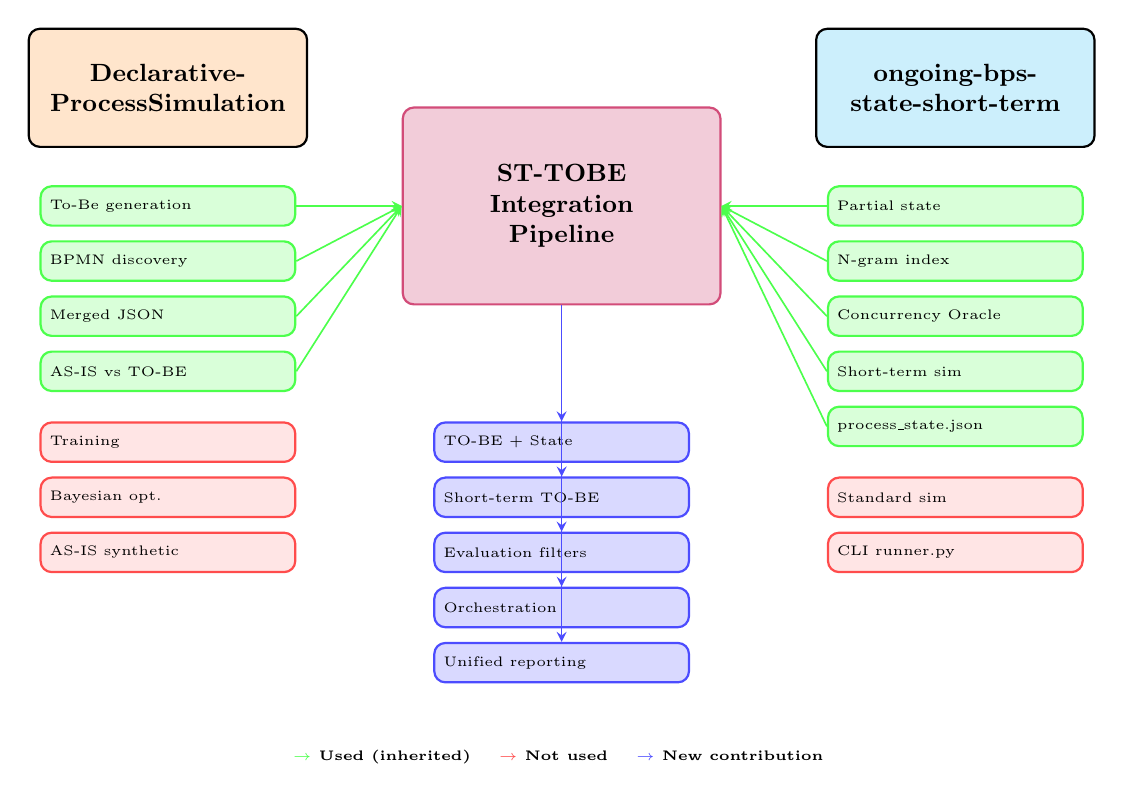
\begin{tikzpicture}[
    node distance=0.8cm and 1.2cm,
    module/.style={rectangle, rounded corners, draw=black, thick,
                   minimum width=3.5cm, minimum height=1.5cm,
                   text width=3.3cm, align=center, font=\small\bfseries},
    used/.style={rectangle, rounded corners, draw=green!70, fill=green!15, thick,
                 minimum width=3.2cm, minimum height=0.5cm,
                 text width=3cm, align=left, font=\tiny},
    notused/.style={rectangle, rounded corners, draw=red!70, fill=red!10, thick,
                    minimum width=3.2cm, minimum height=0.5cm,
                    text width=3cm, align=left, font=\tiny},
    new/.style={rectangle, rounded corners, draw=blue!70, fill=blue!15, thick,
                minimum width=3.2cm, minimum height=0.5cm,
                text width=3cm, align=left, font=\tiny},
    sttobe/.style={rectangle, rounded corners, draw=purple!70, fill=purple!20, thick,
                   minimum width=4cm, minimum height=2.5cm,
                   text width=3.8cm, align=center, font=\small\bfseries},
    arrow/.style={->, >=stealth, semithick},
    label/.style={font=\tiny\bfseries, align=center}
  ]
    
    % DeclarativeProcessSimulation module (left)
    \node[module, fill=orange!20] (declarative) at (-5, 0) {
      Declarative-\\
      ProcessSimulation
    };
    
    % Used components from Declarative (green)
    \node[used] (d1) at (-5, -1.5) {To-Be generation};
    \node[used] (d2) at (-5, -2.2) {BPMN discovery};
    \node[used] (d3) at (-5, -2.9) {Merged JSON};
    \node[used] (d4) at (-5, -3.6) {AS-IS vs TO-BE};
    
    % Not used components from Declarative (red)
    \node[notused] (d5) at (-5, -4.5) {Training};
    \node[notused] (d6) at (-5, -5.2) {Bayesian opt.};
    \node[notused] (d7) at (-5, -5.9) {AS-IS synthetic};
    
    % Ongoing module (right)
    \node[module, fill=cyan!20] (ongoing) at (5, 0) {
      ongoing-bps-\\
      state-short-term
    };
    
    % Used components from Ongoing (green)
    \node[used] (o1) at (5, -1.5) {Partial state};
    \node[used] (o2) at (5, -2.2) {N-gram index};
    \node[used] (o3) at (5, -2.9) {Concurrency Oracle};
    \node[used] (o4) at (5, -3.6) {Short-term sim};
    \node[used] (o5) at (5, -4.3) {process\_state.json};
    
    % Not used components from Ongoing (red)
    \node[notused] (o6) at (5, -5.2) {Standard sim};
    \node[notused] (o7) at (5, -5.9) {CLI runner.py};
    
    % ST-TOBE center module
    \node[sttobe] (sttobe) at (0, -1.5) {
      ST-TOBE\\
      Integration\\
      Pipeline
    };
    
    % New components (blue)
    \node[new] (n1) at (0, -4.5) {TO-BE + State};
    \node[new] (n2) at (0, -5.2) {Short-term TO-BE};
    \node[new] (n3) at (0, -5.9) {Evaluation filters};
    \node[new] (n4) at (0, -6.6) {Orchestration};
    \node[new] (n5) at (0, -7.3) {Unified reporting};
    
    % Arrows from Declarative to ST-TOBE (used components)
    \draw[arrow, green!70] (d1.east) -- (sttobe.west);
    \draw[arrow, green!70] (d2.east) -- (sttobe.west);
    \draw[arrow, green!70] (d3.east) -- (sttobe.west);
    \draw[arrow, green!70] (d4.east) -- (sttobe.west);
    
    % Arrows from Ongoing to ST-TOBE (used components)
    \draw[arrow, green!70] (o1.west) -- (sttobe.east);
    \draw[arrow, green!70] (o2.west) -- (sttobe.east);
    \draw[arrow, green!70] (o3.west) -- (sttobe.east);
    \draw[arrow, green!70] (o4.west) -- (sttobe.east);
    \draw[arrow, green!70] (o5.west) -- (sttobe.east);
    
    % Arrows from ST-TOBE to new components
    \draw[arrow, blue!70] (sttobe.south) -- (n1.north);
    \draw[arrow, blue!70] (sttobe.south) -- (n2.north);
    \draw[arrow, blue!70] (sttobe.south) -- (n3.north);
    \draw[arrow, blue!70] (sttobe.south) -- (n4.north);
    \draw[arrow, blue!70] (sttobe.south) -- (n5.north);
    
    % Legend
    \node[label] (legend) at (0, -8.5) {
      \begin{tabular}{@{}l@{}}
        \textcolor{green!70}{$\rightarrow$} Used (inherited) \quad
        \textcolor{red!70}{$\rightarrow$} Not used \quad
        \textcolor{blue!70}{$\rightarrow$} New contribution
      \end{tabular}
    };
    
  \end{tikzpicture}
  \caption{Component inheritance, exclusion, and novel contributions in ST-TOBE.
           Green arrows indicate components inherited from DeclarativeProcessSimulation (left) and ongoing-bps-state-short-term (right).
           Red items show components not reused.
           Blue items represent novel contributions introduced by ST-TOBE.}
  \label{fig:component_inheritance}
\end{figure}

%========================================
\section{ShortTerm Declarative To-Be integration}
\label{sec:integration}
%========================================

The \emph{shorterm/con-to-be} module orchestrates the
interaction between \emph{DeclarativeProcessSimulation} and
\emph{ongoing-bps-state-short-term}, and adds a dedicated
short-term evaluation and visualisation layer.
It serves as the execution driver for the ST-TOBE pipeline,
while the white-box specification of the complete system (including
data contracts, configuration parameters, and architectural details)
is documented in this article.

\subsection{End-to-end orchestration}

The main entry point, \verb|run_complete_integration.py|,
executes four phases whose automated actions are summarised in
Table~\ref{tbl:orchestration_phases}.

\begin{table}[width=.95\linewidth,cols=2,pos=t]
\caption{Automated phases executed by \texttt{run\_complete\_integration.py}.}
\label{tbl:orchestration_phases}
\begin{tabular*}{\tblwidth}{@{} p{0.3\textwidth} p{0.6\textwidth} @{}}
\toprule
Phase & Automated actions and scripts \\
\midrule
Declarative pipeline & Changes into \verb|DeclarativeProcessSimulation|, activates the required Python environment, and runs the declarative pipeline script so that hallucination, BPMN discovery, JSON merging, and AS-IS/TO-BE simulations are performed before handing artifacts to the integration layer. \\
Ongoing-state and short-term simulation & Locates the most recent TO-BE BPMN and merged JSON under \verb|data/3.bps_tobe/<log_name>/|, then calls \verb|test_ongoing_only.py| to trigger the \emph{ongoing-bps-state-short-term} module, compute the partial state, and launch short-term Prosimos runs with a horizon computed at runtime (e.g., 7 days from the cut-off). \\
Short-term evaluation & Invokes \verb|evaluate_short_term_results.py| so that evaluation utilities from \emph{ongoing-bps-state-short-term} compare the simulated log against \verb|*_ongoing.csv| (or the original log if needed) with event, ongoing, and completion filters for the selected horizon. \\
Comparison and visualisation & Returns to \verb|DeclarativeProcessSimulation/comparison_stats| to regenerate AS-IS vs TO-BE KPI deltas, plots, and HTML reports, ensuring that long-horizon artefacts are aligned with the newly computed short-term evidence. \\
\bottomrule
\end{tabular*}
\end{table}

A final step, \verb|generate_integration_report()|, checks
the presence of key artifacts from each phase and writes a
JSON report summarising their statuses and locations.
The orchestration implements error handling where phases 2 and 3
(ongoing-state and short-term evaluation) may fail without
stopping the pipeline, while phases 1 and 4 (declarative pipeline
and comparison) are mandatory and will halt execution on failure.

Figure~\ref{fig:orchestration} illustrates the execution flow
and error handling strategy of the orchestration pipeline.

\begin{figure}[H]
  \centering
  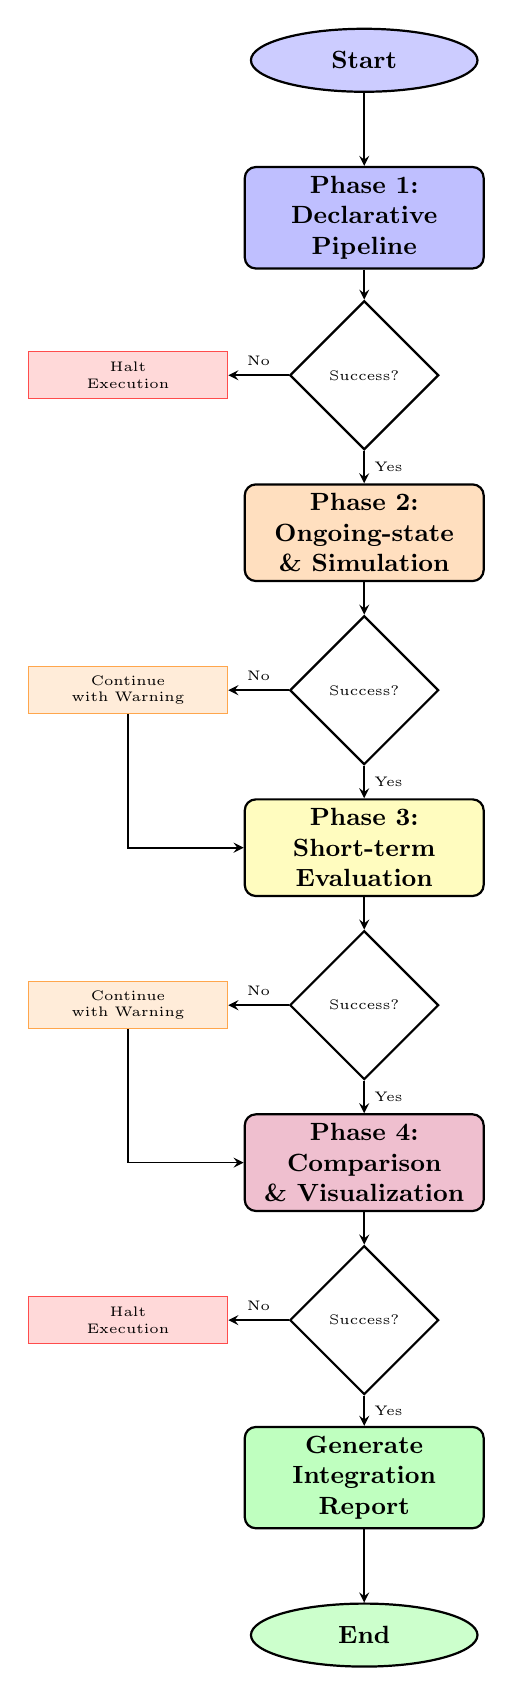
\begin{tikzpicture}[
    node distance=1.2cm and 2cm,
    phase/.style={rectangle, rounded corners, draw=black, thick,
                   minimum width=3cm, minimum height=1.2cm,
                   text width=2.8cm, align=center, font=\small\bfseries},
    decision/.style={diamond, draw=black, thick,
                     minimum width=1.5cm, minimum height=1.5cm,
                     text width=1.3cm, align=center, font=\tiny},
    start/.style={ellipse, draw=black, thick, fill=blue!20,
                  minimum width=2cm, minimum height=0.8cm,
                  text width=1.8cm, align=center, font=\small\bfseries},
    end/.style={ellipse, draw=black, thick, fill=green!20,
                minimum width=2cm, minimum height=0.8cm,
                text width=1.8cm, align=center, font=\small\bfseries},
    error/.style={rectangle, draw=red!70, fill=red!15,
                  minimum width=2.5cm, minimum height=0.6cm,
                  text width=2.3cm, align=center, font=\tiny},
    success/.style={rectangle, draw=green!70, fill=green!15,
                    minimum width=2.5cm, minimum height=0.6cm,
                    text width=2.3cm, align=center, font=\tiny},
    warning/.style={rectangle, draw=orange!70, fill=orange!15,
                    minimum width=2.5cm, minimum height=0.6cm,
                    text width=2.3cm, align=center, font=\tiny},
    arrow/.style={->, >=stealth, semithick}
  ]
    
    % Start node
    \node[start] (start) at (0, 0) {Start};
    
    % Phase 1: Declarative pipeline
    \node[phase, fill=blue!25] (phase1) at (0, -2) {Phase 1:\\Declarative\\Pipeline};
    \node[decision] (check1) at (0, -4) {Success?};
    \node[error] (error1) at (-3, -4) {Halt\\Execution};
    
    % Phase 2: Ongoing-state
    \node[phase, fill=orange!25] (phase2) at (0, -6) {Phase 2:\\Ongoing-state\\\& Simulation};
    \node[decision] (check2) at (0, -8) {Success?};
    \node[warning] (warn2) at (-3, -8) {Continue\\with Warning};
    
    % Phase 3: Short-term evaluation
    \node[phase, fill=yellow!25] (phase3) at (0, -10) {Phase 3:\\Short-term\\Evaluation};
    \node[decision] (check3) at (0, -12) {Success?};
    \node[warning] (warn3) at (-3, -12) {Continue\\with Warning};
    
    % Phase 4: Comparison
    \node[phase, fill=purple!25] (phase4) at (0, -14) {Phase 4:\\Comparison\\\& Visualization};
    \node[decision] (check4) at (0, -16) {Success?};
    \node[error] (error4) at (-3, -16) {Halt\\Execution};
    
    % Final report
    \node[phase, fill=green!25] (report) at (0, -18) {Generate\\Integration\\Report};
    \node[end] (end) at (0, -20) {End};
    
    % Arrows
    \draw[arrow] (start) -- (phase1);
    \draw[arrow] (phase1) -- (check1);
    \draw[arrow] (check1) -- node[above, font=\tiny] {No} (error1);
    \draw[arrow] (check1) -- node[right, font=\tiny] {Yes} (phase2);
    
    \draw[arrow] (phase2) -- (check2);
    \draw[arrow] (check2) -- node[above, font=\tiny] {No} (warn2);
    \draw[arrow] (check2) -- node[right, font=\tiny] {Yes} (phase3);
    \draw[arrow] (warn2) |- (phase3);
    
    \draw[arrow] (phase3) -- (check3);
    \draw[arrow] (check3) -- node[above, font=\tiny] {No} (warn3);
    \draw[arrow] (check3) -- node[right, font=\tiny] {Yes} (phase4);
    \draw[arrow] (warn3) |- (phase4);
    
    \draw[arrow] (phase4) -- (check4);
    \draw[arrow] (check4) -- node[above, font=\tiny] {No} (error4);
    \draw[arrow] (check4) -- node[right, font=\tiny] {Yes} (report);
    
    \draw[arrow] (report) -- (end);
    
  \end{tikzpicture}
  \caption{Execution flow of the ST-TOBE orchestration pipeline.
           Phases 1 and 4 are mandatory (execution halts on failure),
           while phases 2 and 3 are optional (execution continues with warnings on failure).
           The final step generates an integration report summarizing all phases.}
  \label{fig:orchestration}
\end{figure}
\FloatBarrier

\subsection{Short-term evaluation of TO-BE models}

The script \verb|evaluate_short_term_results.py| implements a
log-based evaluation of the short-term simulation by leveraging
evaluation functionality from \emph{ongoing-bps-state-short-term}.
The function \verb|evaluate_short_term_simulation()|:

Table~\ref{tbl:evaluation_steps} details the internal steps executed
by this routine.

\begin{table}[width=.95\linewidth,cols=2,pos=t]
\caption{Steps performed by \texttt{evaluate\_short\_term\_simulation()}.}
\label{tbl:evaluation_steps}
\begin{tabular*}{\tblwidth}{@{} p{0.32\textwidth} p{0.55\textwidth} @{}}
\toprule
Step & Description \\
\midrule
Log ingestion and normalisation & Loads both the reference and simulated logs, applies flexible column mappings, and normalises them to the canonical schema (\texttt{case\_id}, \texttt{activity}, \texttt{resource}, \texttt{start\_time}, \texttt{end\_time}). \\
Cut-off extraction & Reads \verb|last_case_arrival| from \verb|process_state.json|, or derives the cut-off as the maximum \verb|start_time| seen in the reference log when the field is absent. \\
Horizon calculation & Adds the configured \verb|horizon_days| (default 7) to the cut-off timestamp in order to define the end of the short-term evaluation window. \\
Filter partitioning & Splits the aligned logs into paired subsets (\texttt{A\_event}/\texttt{G\_event}, \texttt{A\_ongoing}/\texttt{G\_ongoing}, \texttt{A\_complete}/\texttt{G\_complete}) that correspond to the event, ongoing, and completion filters described in Figure~\ref{fig:evaluation_filters}. \\
\bottomrule
\end{tabular*}
\end{table}

For each subset pair, metrics are computed to quantify how closely the
simulated behaviour matches the reference.
The results, including counts of ongoing and completed cases
and filter-specific metrics (precision, recall, F1-score),
are stored in \verb|evaluation_results.json| and auxiliary
CSV files (one per subset: \verb|A_event_filter.csv|,
\verb|A_ongoing.csv|, \verb|A_complete.csv|, and their
simulated counterparts \verb|G_*|).

Figure~\ref{fig:evaluation_filters} illustrates how the evaluation
process partitions logs into subsets and computes metrics for each filter.

\begin{figure}[H]
  \centering
  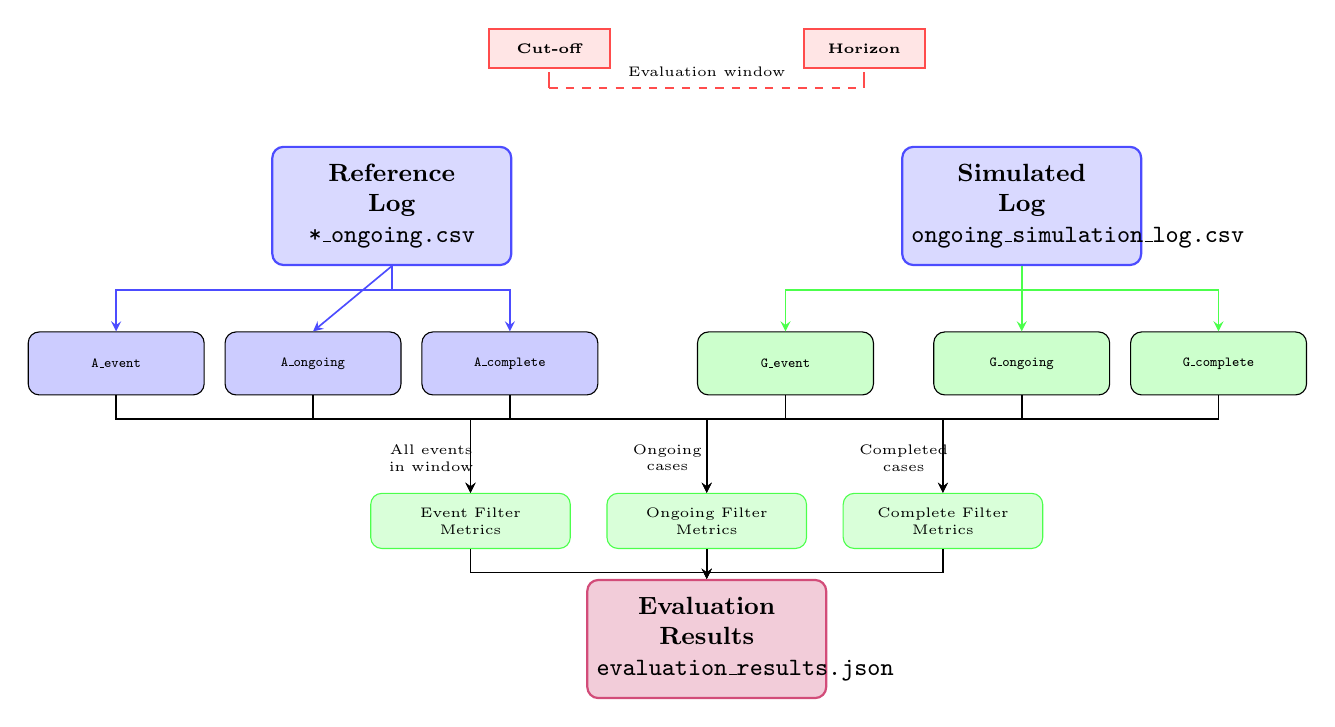
\begin{tikzpicture}[
    node distance=0.8cm and 1.5cm,
    log/.style={rectangle, rounded corners, draw=blue!70, fill=blue!15, thick,
                minimum width=3cm, minimum height=1.5cm,
                text width=2.8cm, align=center, font=\small\bfseries},
    subset/.style={rectangle, rounded corners, draw=black, fill=gray!10,
                   minimum width=2.2cm, minimum height=0.8cm,
                   text width=2cm, align=center, font=\tiny},
    metric/.style={rectangle, rounded corners, draw=green!70, fill=green!15,
                   minimum width=2.5cm, minimum height=0.7cm,
                   text width=2.3cm, align=center, font=\tiny},
    time/.style={rectangle, draw=red!70, fill=red!10, thick,
                 minimum width=1.5cm, minimum height=0.5cm,
                 text width=1.3cm, align=center, font=\tiny\bfseries},
    arrow/.style={->, >=stealth, semithick},
    brace/.style={decorate, decoration={brace, amplitude=5pt, mirror}}
  ]
    
    % Time axis at top
    \node[time] (cutoff) at (-2, 3.5) {Cut-off};
    \node[time] (horizon) at (2, 3.5) {Horizon};
    \draw[thick, red!70] (-2, 3.2) -- (-2, 3);
    \draw[thick, red!70] (2, 3.2) -- (2, 3);
    \draw[thick, red!70, dashed] (-2, 3) -- (2, 3);
    \node[font=\tiny] at (0, 3.2) {Evaluation window};
    
    % Reference log (left side)
    \node[log] (ref-log) at (-4, 1.5) {Reference\\Log\\\texttt{*\_ongoing.csv}};
    
    % Simulated log (right side)
    \node[log] (sim-log) at (4, 1.5) {Simulated\\Log\\\texttt{ongoing\_simulation\_log.csv}};
    
    % Subsets from reference log (left side, below)
    \node[subset, fill=blue!20] (A-event) at (-7.5, -0.5) {\texttt{A\_event}};
    \node[subset, fill=blue!20] (A-ongoing) at (-5, -0.5) {\texttt{A\_ongoing}};
    \node[subset, fill=blue!20] (A-complete) at (-2.5, -0.5) {\texttt{A\_complete}};
    
    % Subsets from simulated log (right side, below)
    \node[subset, fill=green!20] (G-event) at (1, -0.5) {\texttt{G\_event}};
    \node[subset, fill=green!20] (G-ongoing) at (4, -0.5) {\texttt{G\_ongoing}};
    \node[subset, fill=green!20] (G-complete) at (6.5, -0.5) {\texttt{G\_complete}};
    
    % Metrics boxes (bottom)
    \node[metric] (metric-event) at (-3, -2.5) {Event Filter\\Metrics};
    \node[metric] (metric-ongoing) at (0, -2.5) {Ongoing Filter\\Metrics};
    \node[metric] (metric-complete) at (3, -2.5) {Complete Filter\\Metrics};
    
    % Final results
    \node[log, fill=purple!20, draw=purple!70] (results) at (0, -4) {Evaluation\\Results\\\texttt{evaluation\_results.json}};
    
    % Arrows from logs to subsets
    \draw[arrow, blue!70] (ref-log.south) -- ++(0,-0.3) -| (A-event.north);
    \draw[arrow, blue!70] (ref-log.south) -- (A-ongoing.north);
    \draw[arrow, blue!70] (ref-log.south) -- ++(0,-0.3) -| (A-complete.north);
    
    \draw[arrow, green!70] (sim-log.south) -- ++(0,-0.3) -| (G-event.north);
    \draw[arrow, green!70] (sim-log.south) -- (G-ongoing.north);
    \draw[arrow, green!70] (sim-log.south) -- ++(0,-0.3) -| (G-complete.north);
    
    % Arrows from subsets to metrics
    \draw[arrow] (A-event.south) -- ++(0,-0.3) -| (metric-event.north);
    \draw[arrow] (G-event.south) -- ++(0,-0.3) -| (metric-event.north);
    
    \draw[arrow] (A-ongoing.south) -- ++(0,-0.3) -| (metric-ongoing.north);
    \draw[arrow] (G-ongoing.south) -- ++(0,-0.3) -| (metric-ongoing.north);
    
    \draw[arrow] (A-complete.south) -- ++(0,-0.3) -| (metric-complete.north);
    \draw[arrow] (G-complete.south) -- ++(0,-0.3) -| (metric-complete.north);
    
    % Arrows from metrics to results
    \draw[arrow] (metric-event.south) -- ++(0,-0.3) -| (results.north);
    \draw[arrow] (metric-ongoing.south) -- (results.north);
    \draw[arrow] (metric-complete.south) -- ++(0,-0.3) -| (results.north);
    
    % Labels for filter types
    \node[font=\tiny, align=center] at (-3.5, -1.7) {All events\\in window};
    \node[font=\tiny, align=center] at (-0.5, -1.7) {Ongoing\\cases};
    \node[font=\tiny, align=center] at (2.5, -1.7) {Completed\\cases};
    
  \end{tikzpicture}
  \caption{Short-term evaluation process with log-based filters.
           Both reference and simulated logs are partitioned into three subsets each:
           \texttt{A\_event}/\texttt{G\_event} (all events in the evaluation window),
           \texttt{A\_ongoing}/\texttt{G\_ongoing} (cases ongoing at cut-off),
           and \texttt{A\_complete}/\texttt{G\_complete} (cases completing within the horizon).
           Metrics (precision, recall, F1-score) are computed for each filter pair
           and aggregated into \texttt{evaluation\_results.json}.}
  \label{fig:evaluation_filters}
\end{figure}
\FloatBarrier

\subsection{Integration with AS-IS vs TO-BE comparison}

In addition to the short-term evaluation, the module
reuses the AS-IS vs TO-BE comparison results from the
DeclarativeProcessSimulation module:

\begin{table}[width=.95\linewidth,cols=2,pos=t]
\caption{Artifacts reused from \texttt{DeclarativeProcessSimulation/comparison\_stats}.}
\label{tbl:comparison_artifacts}
\begin{tabular*}{\tblwidth}{@{} p{0.35\textwidth} p{0.5\textwidth} @{}}
\toprule
Artifact & Purpose inside shorterm/con-to-be \\
\midrule
Comparison CSV files & Provide KPI deltas (cycle time, waiting time, utilisation, etc.) that contextualise the short-term metrics with long-horizon trends. \\
Performance and change plots & Supply visual evidence (bar charts, radar plots, change curves) that can be embedded into the integration report alongside the new short-term findings. \\
HTML summary report & Acts as a ready-to-share narrative artifact that combines AS-IS vs TO-BE statistics, now referenced by the runtime evaluation layer. \\
\bottomrule
\end{tabular*}
\end{table}

By combining these long-horizon statistics with short-term
evaluation metrics, the ST-TOBE pipeline provides a
holistic picture of the impact of declarative rules:
both in steady-state (AS-IS vs TO-BE simulation) and in the
immediate future (short-term behaviour from the current state).

\subsection{Novel integration mechanisms}

Beyond the orchestration, evaluation, and comparison layers described above,
ST-TOBE introduces several integration mechanisms that did not exist in either
DeclarativeProcessSimulation or ongoing-bps-state-short-term when operating independently.
These mechanisms, illustrated in Figure~\ref{fig:component_inheritance}, enable the unified
runtime To-Be analysis workflow:

\begin{itemize}
  \item \textbf{TO-BE + State integration}: The core novelty is connecting TO-BE model generation
  (from DeclarativeProcessSimulation) with partial state reconstruction (from ongoing-bps-state-short-term).
  Previously, DeclarativeProcessSimulation produced TO-BE models but had no mechanism to evaluate
  their short-term behaviour from a runtime state. Similarly, ongoing-bps-state-short-term could
  reconstruct partial states and simulate short-term, but only for AS-IS models. ST-TOBE bridges
  this gap by using the TO-BE BPMN and merged JSON files as inputs to the state reconstruction engine,
  enabling short-term simulation over future-oriented designs.
  
  \item \textbf{Short-term TO-BE simulation}: While ongoing-bps-state-short-term supported short-term
  simulation from partial state, it was limited to AS-IS models. ST-TOBE extends this capability to
  TO-BE models by: (i) locating the most recent TO-BE artifacts (BPMN and merged JSON) from
  DeclarativeProcessSimulation outputs, (ii) using these artifacts as the process model for state
  reconstruction, and (iii) executing Prosimos short-term simulation with the TO-BE structure while
  preserving AS-IS resource and timing parameters. This allows evaluating how declarative changes
  affect immediate future behaviour, not just long-horizon steady-state.
  
  \item \textbf{Automated artifact retrieval}: The integration automatically selects the most recent
  timestamped TO-BE directory under \verb|data/3.bps_tobe/<log_name>/|, validates the presence of
  required files (\verb|<log_name>.bpmn| and \verb|<log_name>_merged.json|), and handles errors
  gracefully. This eliminates manual intervention and ensures that state reconstruction always uses
  the latest TO-BE artifacts generated by the declarative pipeline.
  
  \item \textbf{Cross-pipeline log reuse}: ST-TOBE reuses \verb|*_ongoing.csv| logs (truncated at
  the cut-off time) that are produced during the declarative pipeline phase. These logs enable
  consistent inference of partial state under TO-BE dynamics, bridging the offline To-Be generation
  phase with the runtime state reconstruction phase. The same log that drives TO-BE discovery is
  reused to compute the partial state, ensuring temporal alignment.
  
  \item \textbf{Unified reporting layer}: The integration combines long-horizon AS-IS vs TO-BE
  comparison statistics (from DeclarativeProcessSimulation) with short-term evaluation metrics
  (from ongoing-bps-state-short-term) into a single reporting framework. The \verb|generate_integration_report()|
  function consolidates status and file locations from all pipeline phases into a JSON report,
  while the comparison and visualization scripts produce HTML reports that reference both long-horizon
  and short-term findings. This unified view enables stakeholders to assess both the steady-state
  impact of declarative changes and their immediate runtime effects.
\end{itemize}

These mechanisms collectively transform previously independent processing streams into a unified
runtime prescriptive-simulation workflow that links long-horizon To-Be analysis with short-term
predictive realism.

%========================================
\section{White-box specification}
\label{sec:whitebox}
%========================================

This section consolidates the white-box specification of the ST-TOBE
pipeline, summarising the main
configuration parameters, data contracts, and extension points
across its modules.
The specification is provided through this documentation, while
the \emph{shorterm/con-to-be} module focuses on orchestration and
execution.

\subsection{Configuration parameters and data contracts}

The ST-TOBE pipeline relies on explicit configuration parameters
and data contracts that enable interoperability between modules.
Key configuration dimensions include: deep generative model settings
(log column mappings, model type, hyperparameters), declarative rules
(encoded in \verb|rules.ini| files), BPMN discovery parameters (Simod
YAML configurations), ongoing-state settings (cut-off time, concurrency
thresholds, N-gram limits), short-term simulation options (horizon
length, Prosimos parameters), and evaluation parameters (filters,
metrics).

Data contracts are defined through standard file formats:
event logs (CSV with canonical columns: \verb|case_id|, \verb|activity|,
\verb|resource|, \verb|start_time|, \verb|end_time|), declarative rules
(INI format), simulation parameters (JSON with arrival distributions,
resource profiles, task-resource mappings), partial state (JSON with
\verb|last_case_arrival| and per-case state structures), and evaluation
results (JSON/CSV with metrics and filtered log subsets).

These structured contracts promote reproducibility and enable
alternative implementations (e.g., different generative models or
state reconstruction strategies) as long as they adhere to the
same input/output formats.
Detailed configuration tables and file format specifications are
provided in Appendix~\ref{app:declarative_module} and
Appendix~\ref{app:ongoing_module}.

\subsection{Extensibility points}

The architecture supports extensibility at multiple levels:
neural network architectures can be extended by adding new generative
models, declarative rule types can be extended by implementing new
rule patterns, additional simulators can be integrated via Docker
wrappers, evaluation metrics and filters can be added to the
short-term evaluation layer, and state-reconstruction strategies
can be replaced as long as they produce the same \verb|process_state.json|
schema.

%========================================
\section{Discussion}
\label{sec:discussion}
%========================================

The ST-TOBE pipeline illustrates how an existing ecosystem of
tools---deep generative models, declarative constraint
handlers, BPMN discovery and simulation engines, ongoing-state
reconstruction modules \citep{ChapelaCampa2025TSC}, and evaluation frameworks---can be
combined into a coherent runtime To-Be analysis workflow
\citep{Meneghello2025IS,Avramenko2025arXiv}.

Several limitations should be noted:

\begin{table}[width=.95\linewidth,cols=2,pos=t]
\caption{Current limitations of the ST-TOBE specification.}
\label{tbl:limitations}
\begin{tabular*}{\tblwidth}{@{} p{0.35\textwidth} p{0.55\textwidth} @{}}
\toprule
Limitation & Practical implication \\
\midrule
Dependence on generative quality & Hallucinated logs inherit biases from the LSTM/GRU models and \verb|rules.ini| expressiveness; overly strict rules can contradict log statistics, degrading downstream BPMN discovery and merged parameters. \\
Approximate state reconstruction & N-gram indices and concurrency heuristics \citep{ChapelaCampa2025TSC} may mis-estimate markings for highly concurrent or unstructured traces, affecting the accuracy of the initial state handed to Prosimos. \\
Sensitivity to evaluation window & Short-term metrics vary with the chosen horizon and with the volume of evidence inside the reference window; sparse windows lead to high variance in precision/recall figures. \\
Single-intervention assumption & The current JSON schemas and simulators model one intervention type with homogeneous resources; supporting multi-policy scenarios would require extending the parameter schema and simulator wrappers. \\
\bottomrule
\end{tabular*}
\end{table}

Despite these limitations, the pipeline offers a transparent
framework for studying how declarative changes and To-Be models
affect short-term behaviour, and for integrating runtime
information into To-Be analysis.

%========================================
\section{Conclusion}
\label{sec:conclusion}
%========================================

This article has presented a white-box specification of the
\emph{ShortTerm Declarative To-Be Integration Pipeline}
(ST-TOBE), an architecture that connects
\emph{DeclarativeProcessSimulation},
\emph{ongoing-bps-state-short-term}, and a dedicated
short-term evaluation layer in a unified workflow.

By making the internal data flow, configuration parameters,
and file contracts explicit, we have shown how:

\begin{enumerate}
  \item deep generative models and declarative rules can be
  used to derive To-Be BPMN models and simulation parameters;
  \item ongoing-state reconstruction can map real-time logs
  onto partial states of To-Be models; and
  \item short-term simulation and evaluation can 
  quantitatively relate simulated behaviour to observed
  behaviour over a limited horizon.
\end{enumerate}

Future work includes integrating causal-prescriptive components
(e.g., treatment effect estimation and intervention policies) \citep{Shoush2025IS,Shoush2024arXiv},
expanding to multi-intervention settings, and exploring
automated selection of To-Be models based on short-term
performance and conformance metrics \citep{Middelhuis2025IS}.

\printcredits

%% Bibliography style
\bibliographystyle{cas-model2-names}

%% Bibliography database (placeholder)
\bibliography{cas-refs}

\bio{}
Andr\'es Mosquera is a researcher in business process management,
simulation, and AI-driven runtime analysis. His work focuses on
bridging prescriptive process monitoring, discrete-event simulation,
and deep generative models for data-driven what-if and To-Be analysis.
\endbio

\clearpage

%========================================
\appendix
%========================================

\section{DeclarativeProcessSimulation module}
\label{app:declarative_module}

The \emph{DeclarativeProcessSimulation} module realises an
offline pipeline that transforms an event log and a set of
declarative rules into AS-IS and TO-BE BPMN models, and into
simulation outputs for both models.

\subsection{Data structure and directory layout}

The module organises its artifacts under a structured
\verb|data/| directory as shown in Table~\ref{tbl:directory_layout}.

\begin{table}[width=.95\linewidth,cols=2,pos=t]
\caption{Directory structure of the DeclarativeProcessSimulation module.}
\label{tbl:directory_layout}
\begin{tabular*}{\tblwidth}{@{} LL @{}}
\toprule
Directory & Contents \\
\midrule
\verb|data/0.logs/| & Original logs, \verb|rules.ini| files, and derived embedding matrices \\
\verb|data/1.predicton_models/| & Trained LSTM/GRU models, metadata, and copy of AS-IS log used for training \\
\verb|data/2.hallucination_logs/| & Synthetic logs generated from models and filtered by declarative rules \\
\verb|data/2.input_logs/| & Compressed versions of original logs for Simod \\
\verb|data/3.bps_asis/| & Discovered AS-IS BPMN models and parameter JSON files \\
\verb|data/3.bps_tobe/| & Discovered TO-BE BPMN models, parameter JSON files, and merged JSON files \\
\verb|data/4.simulation_results/| & Simulation logs and statistics for AS-IS and TO-BE models, plus comparison outputs \\
\bottomrule
\end{tabular*}
\end{table}

Each log is assigned a \verb|<log_name>| and may be associated
with a \verb|<rule_name>| reflecting the applied declarative
rules.

\subsection{Training deep generative models}

The DeclarativeProcessSimulation module configures and trains deep
generative models on the original event log.
Key parameters are summarised in Table~\ref{tbl:training_params},
and the training outputs are listed in Table~\ref{tbl:training_outputs}.

\begin{table}[width=.95\linewidth,cols=2,pos=t]
\caption{Key configuration parameters for deep generative model training.}
\label{tbl:training_params}
\begin{tabular*}{\tblwidth}{@{} LL @{}}
\toprule
Parameter Category & Details \\
\midrule
Log mapping & Mapping from raw column names (\texttt{Case ID}, \texttt{Activity}, \texttt{lifecycle:transition}, \texttt{Resource}) to canonical names (\texttt{caseid}, \texttt{task}, \texttt{event\_type}, \texttt{user}) \\
Time formatting & Formats for parsing timestamps into a continuous time domain \\
Model hyperparameters & Model type (\texttt{shared\_cat}, \texttt{concatenated}), embedding sizes, LSTM layer sizes (\texttt{l\_size}), n-gram sizes (\texttt{n\_size}), optimisation method (e.g., Bayesian optimisation), and number of evaluations (\texttt{max\_eval}) \\
\bottomrule
\end{tabular*}
\end{table}

\begin{table}[width=.9\linewidth,cols=2,pos=t]
\caption{Artifacts produced by the training phase.}
\label{tbl:training_outputs}
\begin{tabular*}{\tblwidth}{@{} LL @{}}
\toprule
Artifact & Description \\
\midrule
Keras/TensorFlow model & Model file (\verb|*.h5|) containing trained weights and architecture \\
Embedding matrices & Pre-trained embeddings and indices for activities and resources \\
Scaling parameters & Normalisation parameters for input features \\
AS-IS log copy & Reference copy of the original log used for training \\
\bottomrule
\end{tabular*}
\end{table}

These artifacts are grouped into a timestamped folder under
\verb|data/1.predicton_models/<log_name>/|.

\subsection{Declarative hallucination and log generation}

The DeclarativeProcessSimulation module instantiates a 
predictor over the trained models and generates
synthetic traces (``hallucinations'') that are post-filtered by
declarative rules.

Rules are read from \verb|rules.ini| files and may constrain
direct succession, eventual succession, forbidden activities,
and required activities, with possible frequency variations.

For each case, the predictor:

\begin{enumerate}
  \item initialises a sequence with padding or a seed n-gram;
  \item repeatedly predicts the next activity (and timestamps),
  applying the rules to prune or enforce specific patterns;
  \item stops when an \emph{End} symbol is generated or a
  maximum length is reached; and
  \item filters out technical activities (e.g., \texttt{Start},
  \texttt{End}) and serialises the resulting trace.
\end{enumerate}

The resulting synthetic log is stored as
\verb|data/2.hallucination_logs/<log_name>/<log_name>.csv|
(and compressed version \verb|.csv.gz|), accompanied by a
configuration file for Simod.

\subsection{BPMN discovery and model merging}

Simod is invoked via Docker wrappers to discover both
AS-IS and TO-BE BPMN models:

\begin{itemize}
  \item For AS-IS, Simod reads the compressed original log and
  \verb|configuration_original.yaml| and outputs
  \verb|<log_name>.bpmn| and \verb|<log_name>.json| under
  \verb|data/3.bps_asis/<log_name>/<run_id>/best_result/|.
  \item For TO-BE, Simod uses the hallucinated log and
  \verb|configuration_generated.yaml| and outputs analogous
  files under \verb|data/3.bps_tobe/<log_name>/<run_id>/best_result/|.
\end{itemize}

Because the To-Be BPMN structure differs from the AS-IS one,
the module performs a \emph{merge} step where tasks are matched
by name between AS-IS and TO-BE BPMN files, simulation fields
(arrival calendars, distributions, resource profiles, task-resource
distributions) from the AS-IS JSON are remapped onto the TO-BE
task identifiers, and a merged JSON file is produced under the TO-BE directory.

The merged JSON thus reflects the TO-BE control-flow structure
while retaining AS-IS resource and timing parameters.

\subsection{Simulation and comparison of AS-IS vs TO-BE}

Prosimos is used (via Docker) to simulate both AS-IS and TO-BE
models.  
For each model, Prosimos consumes the BPMN file and its
corresponding JSON (or merged JSON) and produces:

\begin{itemize}
  \item a simulated event log (\verb|*_prosimos_log.csv|), and
  \item a statistics file (\verb|*_prosimos_stats.csv|) that
  includes overall scenario KPIs (e.g., cycle time, waiting
  time, utilisation).
\end{itemize}

Additionally, BIMP is leveraged through QBP embeddings,
generating alternative simulation log files for integration
with legacy analysis pipelines.

The comparison statistics package reads AS-IS and TO-BE
Prosimos statistics, extracts overall KPIs, and computes
percentage changes, storing the results in comparison CSV files
and generating visual artefacts (bar charts, change analysis plots,
radar plots) and an HTML comparison report.

\section{Ongoing-bps-state-short-term module}
\label{app:ongoing_module}

The \emph{ongoing-bps-state-short-term} module computes the
partial state of a process from an event log truncated at a
given cut-off time and a BPMN model with simulation parameters.
It can also initiate short-term simulations from that state.

\subsection{Inputs, outputs, and architecture}

The module takes three primary inputs and optional inputs as
detailed in Table~\ref{tbl:ongoing_inputs}.
The main output structure is summarised in Table~\ref{tbl:ongoing_outputs}.

\begin{table}[width=.95\linewidth,cols=2,pos=t]
\caption{Inputs to the ongoing-bps-state-short-term module.}
\label{tbl:ongoing_inputs}
\begin{tabular*}{\tblwidth}{@{} LL @{}}
\toprule
Input Type & Description \\
\midrule
\multicolumn{2}{l}{\textbf{Required inputs}} \\
\midrule
Event log (CSV) & The ``ongoing'' log truncated at a cut-off time \\
BPMN 2.0 model & Process model in BPMN format \\
JSON parameters & Stochastic parameters (as produced by Simod or merging step) \\
\midrule
\multicolumn{2}{l}{\textbf{Optional inputs}} \\
\midrule
Column mapping JSON & Custom column name mappings \\
Simulation flags & Flags controlling whether short-term simulation should be executed \\
\bottomrule
\end{tabular*}
\end{table}

\begin{table}[width=.95\linewidth,cols=2,pos=t]
\caption{Output structure of the ongoing-bps-state-short-term module.}
\label{tbl:ongoing_outputs}
\begin{tabular*}{\tblwidth}{@{} LL @{}}
\toprule
Output Component & Description \\
\midrule
\verb|process_state.json| & Main output file containing partial state \\
\verb|last_case_arrival| & Start time of the most recent case \\
Per-case states & Dictionary with the following fields: \\
\midrule
\verb|control_flow_state| & Control-flow marking (flows and activities with tokens) \\
\verb|ongoing_activities| & Activities currently running with resource and timing data \\
\verb|enabled_activities| & Activities that are enabled with enabled times \\
\verb|enabled_gateways| & Gateways that are enabled with enabled times \\
\verb|enabled_events| & Events that are enabled with enabled times \\
\bottomrule
\end{tabular*}
\end{table}

If short-term simulation is enabled, the module also produces a
simulated log and statistics from Prosimos, confined to a given
simulation horizon.

The internal architecture consists of components for input handling,
event log processing, BPMN parsing, state computation, and
short-term simulation execution.

\subsection{Event log ingestion and pre-processing}

The input handling component reads the CSV log, applies column
mapping (if provided) or assumes standard names (\texttt{CaseId},
\texttt{Activity}, \texttt{Resource}, \texttt{StartTime}, \texttt{EndTime}),
converts timestamps to UTC, and loads the BPMN model and JSON parameters.

The event log processor then filters cases that are still ongoing
at the cut-off time (based on \verb|EndTime|), restricts events
to those with \verb|StartTime| not exceeding the cut-off, and
normalises \verb|EndTime| for ongoing events (setting it to \verb|NaT|
as needed).

If \verb|enabled_time| is not present, the module uses a
\emph{Concurrency Oracle} (from \texttt{pix-framework}) to
estimate when each activity was enabled, based on temporal
overlaps and concurrency thresholds.

\subsection{Extended BPMN model, reachability, and N-gram index}

The BPMN handler parses the BPMN XML and extracts tasks,
events, gateways, and sequence flows, then constructs an
\emph{extended} BPMN model by:

\begin{itemize}
  \item replacing each task with a pair \texttt{task+START} and
  \texttt{task+COMPLETE},
  \item inserting an internal flow from the original task node
  through \texttt{+START} to \texttt{+COMPLETE}, and
  \item re-wiring incoming and outgoing flows accordingly.
\end{itemize}

From this extended model, a reachability graph is computed and
used to build an \verb|NGramIndex| with an upper bound on n-gram
length (e.g., 20) \citep{ChapelaCampa2025TSC}.
The index maps sequences of labelled events
(\texttt{TRACE\_START}, \texttt{TaskA+START}, \texttt{TaskA+COMPLETE}, \dots)
to plausible markings in the reachability graph.

\subsection{Case-level state computation}

The state computer processes the pre-processed log grouped
by case.
For each case, it:

\begin{enumerate}
  \item identifies ongoing activities (\verb|EndTime| is
  \verb|NaT|) and collects their IDs, labels, start times,
  resources, and enabled times;
  \item serialises the case history into an event sequence of
  \texttt{+START}/\texttt{+COMPLETE} labels sorted by time;
  \item constructs an n-gram representing the prefix of
  the case, prepending \verb|TRACE_START|;
  \item queries the \verb|NGramIndex| for the best marking
  consistent with the n-gram; and
  \item derives the control-flow state (tokens on flows and
  activities) from the marking.
\end{enumerate}

To reconcile potential discrepancies between the marking and
ongoing activities, the module repairs ``phantom'' activities by
propagating tokens to incoming flows when necessary.

From the marking and repair, the module then:

\begin{itemize}
  \item determines \emph{enabled activities} (targets of flows
  with tokens that lead to tasks),
  \item determines \emph{enabled gateways} (e.g., exclusive
  gateways fed by tokenised flows, but only when upstream tasks
  are not still running), and
  \item determines \emph{enabled events}, excluding end events
  for ongoing analysis.
\end{itemize}

Enabled times are computed by combining information from the
log (e.g., final completion times in the case) and the
concurrency oracle.

\subsection{Short-term simulation from partial state}

The module serialises the set of per-case states and the
\verb|last_case_arrival| field into \verb|process_state.json|.
If short-term simulation is requested, the short-term simulation function
\citep{Avramenko2025arXiv}:

\begin{itemize}
  \item parses the partial state and converts timestamps back
  into datetime objects,
  \item configures Prosimos with the BPMN model, the JSON
  parameters, the partial state, and either a horizon time
  (e.g., 7 days from ``now'') or a total number of cases, and
  \item executes Prosimos to obtain a short-term simulation
  log and statistics.
\end{itemize}

These outputs are saved under
\verb|data/5.ongoing_state/<log_name>/|, including
\verb|process_state.json|,
\verb|ongoing_simulation_log.csv|, and
\verb|ongoing_simulation_stats.csv|.

\end{document}